\chapter{Theoretische Grundlagen und Begriffe}
Dieses Kapitel beinhaltet einen Überblick über Begriffe und Probleme, die in 
dieser Arbeit auftreten.

\section{Graphen und Teilgraphen}
%ToDo: (u,u) nicht erlauben
\begin{mydef}[Graph]Ein Graph $G$ ist ein 2-Tupel $G=(V,E)$. Dabei sind
\begin{itemize}
  \item $V$ eine endliche Menge von Knoten und
  \item $E \subseteq V \times V$ die Menge an Kanten.
\end{itemize}
Ist ein Graph \emph{ungerichtet}, dann gilt für jede Kante $e=(u,v) \in E:
(u,v)=(v,u)$. Im \emph{gerichteten} Fall gilt: $(u,v)\neq (v,u)$.
\end{mydef}

\begin{mydef}[Teilgraph]
Es sei $T=(V_t,E_t)$ ein Graph. $T$ ist Teilgraph des Graphen $G=(V,E)$ genau
dann, wenn die beiden nachfolgenden Bedingungen gelten:
\begin{itemize}
	\item $V_t \subseteq V$ 
	\item $e \in E_t \Rightarrow e \in E$
\end{itemize}
Gilt für alle $u,v \in V_t$ zusätzlich $(u,v) \in E \Rightarrow (u,v) \in E_t$, dann
ist $T$ ein \emph{induzierter} Teilgraph.\end{mydef}

Der Unterschied zwischen einem induzierten und nichtinduzierten 
Teilgraphen liegt darin, dass bei einem induzierten jede Kante 
zwischen zwei Knoten $u$ und $v$ enthalten sein muss ($(u,v) \in E_t 
\Leftrightarrow (u,v) \in E$). Bei einem nichtinduzierten Teilgraph 
ist dies optional ($(u,v) \in E_t \Rightarrow (u,v) \in E$). 
Abbildung \ref{pic:bsp_tg} stellt dies dar. Zwar ist $T$ ein (nichtinduzierter) Teilgraph 
von $G$, jedoch fehlt die Kante $(a,c)$, damit $T$ auch ein induzierter Teilgraph ist.


%\begin{figure}[htb]
%\centering
%\hspace*{\fill}
%\subfloat[]{\includegraphics[width=0.3\linewidth,
%keepaspectratio]{bilder/bsp_tg_g}}
%\hspace*{\fill}
%\subfloat[]{\includegraphics[width=0.3\linewidth,
%keepaspectratio]{bilder/bsp_tg_t}}
%\hspace*{\fill}
%\caption{Der Graph $G$ und dessen Teilgraph $T$}
%\label{pic:bsp_tg}
%\end{figure}

\begin{figure}[htb]
\centering
\hspace*{\fill}
\subfloat[]{\begin{tikzpicture}
  [normalN/.style={circle,draw,minimum size=0.8cm,thick},
   node distance=1.3cm]

  \node[normalN] (a) {a};
    
  \node[normalN] (b) [right=of a] {b}
    edge [thick] (a);
    
  \node[normalN] (c) [below=of b] {c}
    edge [thick] (b)
    edge [thick] (a);
    
  \node[normalN] (d) [left=of c] {d}
    edge [thick] (a)
    edge [thick] (c);

  
\end{tikzpicture}}
\hspace*{\fill}
\subfloat[]{\begin{tikzpicture}
  [normalN/.style={circle,draw,minimum size=0.8cm,thick},
   hiddenN/.style={circle,draw=black!33,black!33,minimum size=0.8cm,thick},
   node distance=1.3cm]

  \node[normalN] (a) {a};
    
  \node[normalN] (b) [right=of a] {b}
    edge [thick] (a);
    
  \node[normalN] (c) [below=of b] {c}
    edge [thick] (b)
    edge [thick,black!33] (a);
    
  \node[hiddenN] (d) [left=of c] {d}
    edge [thick,black!33] (a)
    edge [thick,black!33] (c);
  
\end{tikzpicture}}
\hspace*{\fill}
\caption{Der Graph $G$ und dessen Teilgraph $T$}
\label{pic:bsp_tg}
\end{figure}

\section{Graphisomorphie}
Graphisomorphie (GI) bezeichnet vereinfacht gesagt, ob zwei Graphen gleich
sind. Dies bedeutet bildlich gesprochen, dass man beide Graphen
übereinander legen kann.

\begin{mydef}[Graphisomorphie]
Zwei Graphen $G_1 = (V_1,E_1)$ und $G_2 = (V_2,E_2)$ heißen isomorph, wenn
eine bijektive Abbildung $\varphi: V_1 \rightarrow V_2$ existiert, so dass
für alle $u,v \in V_1$ gilt: $(u,v) \in E_1 \Leftrightarrow (\varphi(u),
\varphi(v)) \in E_2$.
\end{mydef}

Das zur GI gehörende Entscheidungsproblem fragt, ob für zwei gegebene 
Graphen eine oben genannte Abbildung existiert. Eine Besonderheit ist 
hierbei die Komplexität. Zwar liegt GI in NP\footnote{Ein Problem liegt 
in NP genau dann, wenn es mit einer nichtdeterministischen (Turing-)Maschine 
in polynomieller Zeit gelöst werden kann.} \cite{GIinNP}, jedoch konnte bis 
zum Zeitpunkt dieser Arbeit weder bewiesen noch widerlegt werden, ob es 
möglich ist, GI in Polynomialzeit zu lösen oder ob GI NP-vollständig\footnote{Ein 
Problem ist NP-vollständig genau dann, wenn es in NP liegt und sich jedes 
Problem in NP in Polynomialzeit darauf reduzieren lässt.} ist \cite{wikiD:GI,wikiE:GI}. 

Es ist also unbekannt, ob es einen Algorithmus gibt, der 
mit polynomiellem Aufwand überprüft, ob zwei Graphen isomorph sind.


\section{Teilgraphisomorphie}
Ähnlich zur einfachen GI gibt Teilgraphisomorphie (TGI) an, ob ein Graph 
$G_1$ isomorph zu einem Teilgraph von $G_2$ ist.

\begin{mydef}[Teilgraphisomorphie]
Ein Graph $G_1 = (V_1,E_1)$ ist isomorph zu einem Teilgraph von $G_2 =
(V_2,E_2)$ genau dann, wenn eine injektive Abbildung $\varphi: V_1
\rightarrow V_2$ existiert und für alle $u,v \in V_1$ gilt: $(u,v) \in E_1
\Rightarrow (\varphi(u),\varphi(v)) \in E_2$.
\end{mydef}

Analog zur GI wird auch beim TGI-Problem nach der Existenz einer in der 
Definition beschriebenen Abbildung gefragt. Das TGI-Problem ist 
NP-vollständig \cite{Cook:1971}.

\subsubsection{Anmerkung}
Im Rahmen dieser Arbeit wird in dem Fall, dass $G_1$ isomorph zu einem 
Teilgraph von $G_2$ ist, lediglich davon gesprochen, dass $G_1$ ein 
Teilgraph von $G_2$ ist. 


\section{Größter gemeinsamer Teilgraph}
Der größte gemeinsame Teilgraph (engl.: maximum common subgraph) 
zweier Graphen $G_1$ und $G_2$ beschreibt den größtmöglichen Graphen $H$, 
der Teilgraph von $G_1$ und $G_2$ ist.

\begin{mydef}[gemeinsamer Teilgraph (gTG)]\label{def:gTG} 
Ein Graph $H=(V_H,E_H)$ ist ein gemeinsamer Teilgraph von $G_1 = (V_1,E_1)$ und 
$G_2=(V_2,E_2)$ genau dann, wenn alle der vier nachflogenden Bedingungen 
erfüllt sind:
\begin{itemize}
  \item $V_H \subseteq V_1$
  \item $E_H \subseteq E_1$
	\item Es existiert eine injektive Abbildung $\varphi: V_H \rightarrow V_2$
	\item Für alle $u,v \in V_H$ gilt: $(u,v) \in E_H \Rightarrow (\varphi(u),
	      \varphi(v)) \in E_2$
\end{itemize}

Handelt es sich um einen gemeinsamen \emph{induzierten} Teilgraphen (giTG), 
dann gilt zusätzlich für alle $u,v \in V_H$: $(u,v) \in E_1 \Leftrightarrow 
(u,v) \in E_H \Leftrightarrow (\varphi(u),\varphi(v)) \in E_2$
\end{mydef}

\subsection{Der induzierte Fall}
Das Maß für die Größe des Teilgraphen ist abhängig davon, ob 
der giTG betrachtet wird oder lediglich der gTG. Im induzierten 
Fall ist die Anzahl der Knoten von $H$ das Größenmaß.

\begin{mydef}[größter gemeinsamer induzierter Teilgraph]
Sei $H=(V_H,E_H)$ ein giTG von $G_1$ und $G_2$. $H$ ist größter giTG von 
$G_1$ und $G_2$ genau dann, wenn kein giTG $H'=(V',E')$ von $G_1$ und $G_2$ 
existiert mit $|V'|>|V_H|$. Der größte giTG wird als MCS bezeichnet.
\end{mydef}

%\begin{figure}[htb]
%\centering
% %\hfill %
%\subfloat[]{\includegraphics[width=0.4\linewidth,
%keepaspectratio]{bilder/bsp_giTG_g1}}
%\hspace{1.5cm} 
%\subfloat[]{\includegraphics[width=0.4\linewidth,
%keepaspectratio]{bilder/bsp_giTG_g2}}
% %\hfill %
%\caption{Der MCS (blau) zweier Graphen}
%\label{pic:giTG}
%\end{figure}

\begin{figure}[htb]
\centering
\hspace*{\fill}
\subfloat[]{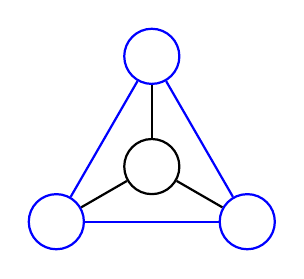
\begin{tikzpicture}
  [normalN/.style={circle,draw,minimum size=0.7cm,thick}]

  \node[normalN]      (center) at (0:0)     {};
  \node[normalN,blue] (top)    at (90:1.4)  {};
  \node[normalN,blue] (left)   at (210:1.4) {};
  \node[normalN,blue] (right)  at (-30:1.4) {};
  
  \draw [thick] (center) -- (top);
  \draw [thick] (center) -- (left);
  \draw [thick] (center) -- (right);
  
  \draw [thick,blue] (left) -- (right);
  \draw [thick,blue] (top) -- (right);
  \draw [thick,blue] (top) -- (left);
  
\end{tikzpicture}}
\hspace*{\fill}
\subfloat[]{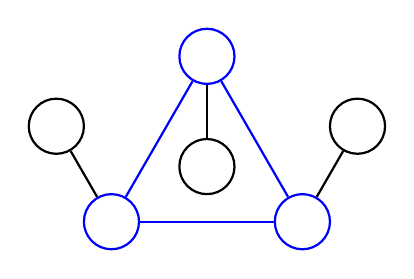
\begin{tikzpicture}
  [normalN/.style={circle,draw,minimum size=0.7cm,thick},
   blueN/.style={normalN,blue}]

  \node[normalN] (center) at (0:0)    {};
  \node[blueN]   (top)    at (90:1.4) {};
  
  \path (210:1.4) node[blueN]   (left) {}
       +(120:1.4) node[normalN] (l)    {};
  

  \path (-30:1.4) node[blueN]   (right) {}
       +(60:1.4)  node[normalN] (r)     {};
  
  \draw [thick] (center) -- (top);
  %\draw [thick] (center) -- (left);
  %\draw [thick] (center) -- (right);
  
  \draw [thick,blue] (left) -- (right);
  \draw [thick,blue] (top) -- (right);
  \draw [thick,blue] (top) -- (left);
  
  \draw [thick] (left)  -- (l);
  \draw [thick] (right) -- (r);
\end{tikzpicture}}
\hspace*{\fill}
\caption{Der MCS (blau) zweier Graphen}
\label{pic:giTG}
\end{figure}

Das NP-vollständige \cite{Garey:1990} MCS-Problem stellt die folgende Frage: 
Existiert für zwei Graphen $G_1=(V_1,E_1)$ und $G_2=(V_2,E_2)$ sowie ein 
$k>0$ ein giTG $H=(V_H,E_H)$, für den gilt: $|V_H| \geq k$?


\subsection{Der allgemeine Fall}
Wird lediglich der gTG betrachtet, ist die Anzahl der Kanten das Maß 
für die Größe. Dies liegt daran, dass ein Graph $H$, der nur aus den 
Knoten des kleineren der Graphen $G_1$ und $G_2$ besteht, immer ein 
gTG von $G_1$ und $G_2$ ist. Zum größten gTG zweier Graphen gehören somit 
immer alle Knoten des kleineren Graphen.


\begin{myTheo}
Gegeben seien zwei Graphen $G_1 = (V_1,E_1)$ und $G_2=(V_2,E_2)$, wobei 
$|V_1| \leq |V_2|$. $H=(V_1,\emptyset)$ ist dann ein gTG von $G_1$ und $G_2$.
\end{myTheo}

\begin{myProof}
$H=(V_H,E_H)=(V_1,\emptyset)$ ist gTG von $G_1$ und $G_2$, wenn die folgenden 
Bedingungen (aus Definition \ref{def:gTG}) gelten:
\begin{enumerate}
  \item $V_H \subseteq V_1$
  \item $E_H \subseteq E_1$
	\item Es existiert eine injektive Abbildung $\varphi: V_H \rightarrow V_2$
	\item Für alle $u,v \in V_H$ gilt: $(u,v) \in E_H \Rightarrow (\varphi(u),
	      \varphi(v)) \in E_2$
\end{enumerate}

Die Bedingungen 1 ($V_1 \subseteq V_1$) und 2 ($\emptyset \subseteq E_1$) sind 
offensichtlich erfüllt.

Bedingung 3: Eine injektive Abbildung lässt sich dadurch erzeugen, dass jedem 
Knoten in $V_1$ ein Knoten in $V_2$ zugewiesen wird. Da $|V_1| \leq |V_2|$ ist 
es möglich jedem Knoten in $V_1$ einen anderen Knoten in $V_2$ zuzuordnen. 
Somit existiert immer eine injektive Abbildung.

Bedingung 4: Da $H$ keine Kanten besitzt ($E_H=\emptyset$), gilt für alle 
$u,v \in V_H$, dass $(u,v) \in E_H$ eine falsche Aussage ist. Somit ist die 
Implikation in Bedingung 4 immer wahr.

Alle Bedingungen sind erfüllt, somit ist $H$ ein gTG von $G_1$ und $G_2$. \qed
\end{myProof}

%\begin{figure}[htb]
%\centering
% %\hfill %
%\subfloat[]{\includegraphics[width=0.4\linewidth,
%keepaspectratio]{bilder/bsp_gTG_g1}}
%\hspace{1.5cm} 
%\subfloat[]{\includegraphics[width=0.4\linewidth,
%keepaspectratio]{bilder/bsp_gTG_g2}}
% %\hfill %
%\caption{Der größte gTG (grün) zweier Graphen}
%\label{pic:gTG}
%\end{figure}

\begin{figure}[htb]
\centering
\hspace*{\fill} 
\subfloat[]{\begin{tikzpicture}
  [normalN/.style={circle,draw,minimum size=0.7cm,thick}]

  \node[normalN,darkgreen] (center) at   (0:0)   {};
  \node[normalN,darkgreen] (top)    at  (90:1.4) {};
  \node[normalN,darkgreen] (left)   at (210:1.4) {};
  \node[normalN,darkgreen] (right)  at (-30:1.4) {};
  
  \draw [thick,darkgreen] (center) -- (top);
  \draw [thick] (center) -- (left);
  \draw [thick] (center) -- (right);
  
  \draw [thick,darkgreen] (left) -- (right);
  \draw [thick,darkgreen] (top) -- (right);
  \draw [thick,darkgreen] (top) -- (left);
  
\end{tikzpicture}}
\hspace*{\fill} 
\subfloat[]{\begin{tikzpicture}
  [normalN/.style={circle,draw,minimum size=0.7cm,thick},
   blueN/.style={normalN,darkgreen}]

  \node[blueN] (center) at (0:0)    {};
  \node[blueN]   (top)    at (90:1.4) {};
  
  \path (210:1.4) node[blueN]   (left) {}
       +(120:1.4) node[normalN] (l)    {};
  

  \path (-30:1.4) node[blueN]   (right) {}
       +(60:1.4)  node[normalN] (r)     {};
  
  \draw [thick,darkgreen] (center) -- (top);
  %\draw [thick] (center) -- (left);
  %\draw [thick] (center) -- (right);
  
  \draw [thick,darkgreen] (left) -- (right);
  \draw [thick,darkgreen] (top) -- (right);
  \draw [thick,darkgreen] (top) -- (left);
  
  \draw [thick] (left)  -- (l);
  \draw [thick] (right) -- (r);
\end{tikzpicture}}
\hspace*{\fill} 
\caption{Der größte gTG (grün) zweier Graphen}
\label{pic:gTG}
\end{figure}

\begin{mydef}[größter gemeinsamer Teilgraph]
Sei $H=(V_H,E_H)$ ein gTG von $G_1$ und $G_2$. $H$ ist größter gTG von 
$G_1$ und $G_2$ genau dann, wenn kein gTG $H'=(V',E')$ 
von $G_1$ und $G_2$ existiert mit $|E'|>|E_H|$
\end{mydef}


\section{Graphabstand}\label{sec:Graphabstand}
Als Graphabstand (engl.: graph edit distance) bezeichnet man die Kosten, 
die nötig sind, um einen Graphen so umzubauen, dass er isomorph zu einem 
anderen ist. 

Die Definitionen in diesem Abschnitt basieren auf den entsprechenden Definitionen 
in \cite{Bunke:1997}.

\begin{mydef}[error correcting graph matching (ECGM)]
Es seien $G_1=(V_1,E_1)$ und $G_2=(V_2,E_2)$ Graphen. Ein 
error correcting graph matching ist eine bijektive Abbildung 
$\varphi:\hat{V}_1 \rightarrow \hat{V}_2$ mit $\hat{V}_1 
\subseteq V_1$ und $\hat{V}_2 \subseteq V_2$.
\end{mydef}

Die Abbildung $\varphi$ stellt nun eine mögliche Bearbeitung von $G_1$ 
zu $G_2$ dar. Aus $G_1$, $G_2$ und $\varphi$ leiten sich ab: 
\begin{itemize}
	\item $V_d:=V_1 \backslash \hat{V}_1$ sind die zu löschenden Knoten,
	\item $V_a:=V_2 \backslash \hat{V}_2$ sind die hinzuzufügenden Knoten,
	\item $E_d:=E_1 \backslash \{(u,v) \ |\ u,v \in \hat{V}_1 \wedge (\varphi(u),
	       \varphi(v)) \in E_2\}$ sind die zu löschenden Kanten und
	\item $E_a:=E_2 \backslash \{(\varphi(u),\varphi(v))\ |\ u,v \in E_1 
	       \backslash E_d\}$ sind die hinzuzufügenden Kanten.
\end{itemize}

\begin{mydef}[Kosten eines ECGM]
Die Kosten eines ECGM $\varphi$ von $G_1$ nach $G_2$ seien definiert durch
\[
c(\varphi)=\sum_{v \in V_d}c_{nd}(v) + \sum_{v \in V_a}c_{na}(v) + 
  \sum_{e \in E_a}c_{ed}(e) + \sum_{e \in E_d}c_{ea}(e).
\]
Dabei seien: 
\begin{itemize}
	\item $c_{nd}(v) \geq 0$ die Kosten für das Löschen eines Knotens,
	\item $c_{na}(v) \geq 0$ die Kosten für das Hinzufügen eines Knotens,
	\item $c_{ed}(e) \geq 0$ die Kosten für das Löschen einer Kante und
	\item $c_{ea}(e) \geq 0$ die Kosten für das Hinzufügen einer Kante.
\end{itemize}
\end{mydef}

Es ist möglich, die Kostenfunktion zu erweitern. Besitzt ein Graph 
beispielsweise eine Beschriftung oder Gewichtung (dies können z.B. 
Entfernungen in einem Straßennetz sein), so ist das Editieren eines 
Knotens oder einer Kante möglich. Dabei entfernt man die Kante nicht, 
sondern ändert lediglich die Beschriftung oder das Gewicht. 

\begin{mydef}[Graphabstand]
Der Graphabstand $d(G_1,G_2)$ für zwei Graphen $G_1$ und $G_2$ sei 
definiert durch die minimalen Kosten über allen möglichen ECGMs von $G_1$ 
nach $G_2$.
\[
d(G_1,G_2):=\min\{c(\varphi)\ |\ \varphi \text{ ist ein ECGM von } G_1 
\text{ nach } G_2\}
\]
\end{mydef}

\subsubsection{Graphabstand als Entscheidungsproblem}
Gegeben seien zwei Graphen $G_1$ und $G_2$ sowie ein $k$. Existiert ein 
ECGM $\varphi$ von $G_1$ nach $G_2$ mit $c(\varphi) \leq k$?

Garaphabstand ist NP-vollständig. \cite{GEDisNPcomp}


\section{Zusammenhang von MCS und Graphabstand}\label{sec:MCS_Graphabstand}
In \cite{Bunke:1997} wird gezeigt, dass bei geeigneter Wahl der Kosten 
der Graphabstand zweier Graphen $G_1=(V_1,E_1)$ und $G_2=(V_2,E_2)$ 
durch die Größe des MCS $G=(V,E)$ berechnet werden kann. Es gilt dann:

\begin{equation}
d(G_1,G_2)=|V_1| + |V_2| - 2 |V|\label{form:mcs}
\end{equation}

Der Graphabstand kann somit ermittelt werden, indem man den MCS zweier 
Graphen bildet. Knoten und Kanten, die nicht zum MCS gehören werden entfernt 
oder hinzugefügt.

Die Kostenfunktionen $c_{nd}(v)$, $c_{na}(v)$, $c_{ed}(e)$, und $c_{ea}(e)$, 
die in \cite{Bunke:1997} angegeben wurden, damit (\ref{form:mcs}) gilt, sind 
(angepasst an die in dieser Arbeit verwendeten Definitionen eines 
Graphen und Kosten eines ECGMs) wie folgt definiert:

\begin{itemize}
	\item $c_{na}(v)=1$
	\item $c_{nd}(v)=1$
	\item $c_{ed}(e)=\left\{\begin{array}{ll}\infty & e \in \hat{V}_1 \times 
	                  \hat{V}_1\\0 & \text{sonst}\end{array}\right. $
	\item $c_{ea}(e)=\left\{\begin{array}{ll}\infty & e \in \hat{V}_2 \times 
	                  \hat{V}_2\\0 & \text{sonst}\end{array}\right. $
\end{itemize}

\subsection{Probleme bei der Nutzung}
Beim Ermitteln des Graphabstands mittels des MCS und der oben beschriebenen 
Kostenfunktion ergeben sich Probleme.

Die Kosten für das Hinzufügen und Entfernen von Kanten sind entweder $0$ oder 
unendlich. Solange der Graphabstand endlich ist, ist er somit unabhängig von 
der Anzahl der Kanten, die hinzugefügt oder entfernt werden müssen.

Ein weiteres Problem ist, dass alle Knoten, die nicht zum MCS gehören, entfernt 
oder hinzugefügt werden. Es kann jedoch Fälle geben, in denen das nicht erwünscht 
ist. Abbildung \ref{pic:bspMCS_GED} stellt einen solchen Fall dar. Der MCS ist 
dabei \emph{grün} markiert.

%\begin{figure}[htb]
%\centering
%\hspace*{\fill} 
%\subfloat[Eingabe des Lerners]{\includegraphics[width=0.25\linewidth,
%keepaspectratio]{bilder/bsp_msc_ged_1}}
%\hspace*{\fill} 
%\subfloat[Musterlösung]{\includegraphics[width=0.25\linewidth,
%keepaspectratio]{bilder/bsp_msc_ged_2}}
%\hspace*{\fill} 
%\caption{Beispiel für einen ungüstigen MCS (grün) zweier Graphen}
%\label{pic:bspMCS_GED}
%\end{figure}

\begin{figure}[htb]
\centering
\hspace*{\fill} 
\subfloat[Eingabe des Lerners]{\begin{tikzpicture}
  [normalN/.style={circle,draw,minimum size=0.8cm,thick},
   greenN/.style={circle,draw=darkgreen,minimum size=0.8cm,thick},
   node distance=1.3cm]

  \node[greenN] (a) {a};
    
  \node[greenN] (b) [right=of a] {b}
    edge [thick,darkgreen] (a);
    
  \node[normalN] (c) [below=of b] {c}
    edge [thick] (b);
    
  \node[greenN] (d) [left=of c] {d}
    edge [thick,darkgreen] (a)
    edge [thick] (c);
  
\end{tikzpicture}}
\hspace*{\fill} 
\subfloat[Musterlösung]{\begin{tikzpicture}
  [normalN/.style={circle,draw,minimum size=0.8cm,thick},
   greenN/.style={circle,draw=darkgreen,minimum size=0.8cm,thick},
   node distance=1.3cm]

  \node[greenN] (a) {1};
    
  \node[greenN] (b) [right=of a] {2}
    edge [thick,darkgreen] (a);
    
  \node[normalN] (c) [below=of b] {3}
    edge [thick] (b)
    edge [thick] (a);
    
  \node[greenN] (d) [left=of c] {4}
    edge [thick,darkgreen] (a)
    edge [thick] (c);
  
\end{tikzpicture}}
\hspace*{\fill} 
\caption{Beispiel für einen ungünstigen MCS (grün) zweier Graphen}
\label{pic:bspMCS_GED}
\end{figure}

Der Fehler des Lerners in Abbildung \ref{pic:bspMCS_GED} ist lediglich eine 
fehlende Kante. Ermittelt man nun den Graphabstand mittels des MCS, so wird 
der Knoten~$c$ entfernt und Knoten~$3$ hinzugefügt. Somit wird Knoten~$c$ als 
fehlerhaft und Knoten~$3$ als fehlend betrachtet.

\subsection{Kantengraphen}
Kantengraphen sind ein für diese Arbeit erdachtes Konzept. Die Idee 
daran ist, in einem gegebenen Graphen die Kanten durch zusätzliche 
Knoten darzustellen. Der Kantengraph $K$ eines Graphen $G=(V,E)$ ergibt 
sich, indem man jede Kante $e=(u,v) \in E$ zur Knotenmenge hinzugefügt 
und der so entstandene Knoten mit den "`alten"' Knoten $u$ und $v$ 
verbunden wird. Abbildung \ref{pic:bspKantengraph} stellt dies dar.

\begin{mydef}[Kantengraph]\label{def:Kantengraph}
Für einen gegebenen Graphen $G=(V,E)$ sei dessen Kantengraph $K$ wie folgt 
definiert: 
\[
K=(V \cup E, \{(u,e),(e,v)\ |\ e=(u,v) \in E\})
\]
Die Funktion $k$ gibt den Kantengraph des übergeben Graphen zurück. 
\[ k(G)=K \]
\end{mydef}

%\begin{figure}[htb]
%\centering
% %\hspace*{\fill} 
%\subfloat[Original]{\includegraphics[width=0.25\linewidth,
%keepaspectratio]{bilder/bspKantengraph_1}}
%\hspace*{\fill} 
%\subfloat[Kanten in Knoten umwandeln]{\includegraphics[width=0.25\linewidth,
%keepaspectratio]{bilder/bspKantengraph_2}}
%\hspace*{\fill} 
%\subfloat[neue Kanten]{\includegraphics[width=0.25\linewidth,
%keepaspectratio]{bilder/bspKantengraph_3}}
% %\hspace*{\fill} 
%\caption{Erstellen eines Kantengraphen}
%\label{pic:bspKantengraph}
%\end{figure}

\begin{figure}[htb]
\centering
%\hspace*{\fill} 
\subfloat[Original]{\begin{tikzpicture}
  [normalN/.style={circle,draw,minimum size=0.8cm,thick},
   node distance=1.3cm]

  \node[normalN] (a) {};
    
  \node[normalN] (b) [right=of a] {}
    edge [thick] (a);
    
  \node[normalN] (c) [below=of b] {}
    edge [thick] (b);
    
  \node[normalN] (d) [left=of c] {}
    edge [thick] (a)
    edge [thick] (c);
  
\end{tikzpicture}}
\hspace*{\fill} 
\subfloat[Kanten in Knoten umwandeln]{\begin{tikzpicture}
  [normalN/.style={circle,draw,minimum size=0.8cm,thick},
   edgeN/.style={draw,minimum size=0.4cm,thick},
   node distance=0.45cm]

  \node[normalN] (a)                {};
  \node[edgeN]   (ab) [right=of a]  {};
  \node[normalN] (b)  [right=of ab] {};

  \node[edgeN]   (ad) [below=of a]  {};
  \node[edgeN]   (bc) [below=of b]  {};

  \node[normalN] (d)  [below=of ad] {};
  \node[edgeN]   (cd) [right=of d]  {};
  \node[normalN] (c)  [right=of cd] {};

\end{tikzpicture}}
\hspace*{\fill} 
\subfloat[neue Kanten]{\begin{tikzpicture}
  [normalN/.style={circle,draw,minimum size=0.8cm,thick},
   edgeN/.style={draw,minimum size=0.4cm,thick},
   node distance=0.45cm]

  \node[normalN] (a)                {};
  \node[edgeN]   (ab) [right=of a]  {};
  \node[normalN] (b)  [right=of ab] {};

  \node[edgeN]   (ad) [below=of a]  {};
  \node[edgeN]   (bc) [below=of b]  {};

  \node[normalN] (d)  [below=of ad] {};
  \node[edgeN]   (cd) [right=of d]  {};
  \node[normalN] (c)  [right=of cd] {};

  \draw[thick,dashed] (a) -- (ab);
  \draw[thick,dashed] (a) -- (ad);
  \draw[thick,dashed] (b) -- (ab);
  \draw[thick,dashed] (b) -- (bc);
  \draw[thick,dashed] (c) -- (bc);
  \draw[thick,dashed] (c) -- (cd);
  \draw[thick,dashed] (d) -- (ad);
  \draw[thick,dashed] (d) -- (cd);
\end{tikzpicture}
}
%\hspace*{\fill} 
\caption{Erstellen eines Kantengraphen}
\label{pic:bspKantengraph}
\end{figure}

Mit Hilfe eines Kantengraphen lassen sich nun die oben genannten 
Probleme umgehen. Dazu sucht man nicht den MCS der ursprünglichen 
Graphen, sondern den MCS der Kantengraphen. Dabei gilt es aber zu 
beachten, dass man Knoten, die eine Kante darstellen und normale 
Knoten nicht einander zuordnet.

Ein Problem der ursprünglichen Graphen war, dass Kanten nicht 
bewertet wurden. Da jede Kante nun als Knoten betrachtet wird, 
wird somit auch jede Kante in die Kosten für den Graphabstand 
eingerechnet. 

Ein weiteres Problem war, dass der MCS ein induzierter Teilgraph ist, 
wodurch Knoten ungewollt als fehlerhaft betrachtet werden können. Dieses 
Problem ist nun nicht mehr relevant, da jeder Teilgraph von $G$ ein 
induzierter Teilgraph von dessen Kantengraph $K$ ist. In dem 
Beispiel aus Abbildung~\ref{pic:bspMCS_GED} würden somit auch 
Knoten $c$ und $3$ zum MCS gehören.

\begin{myTheo}
Wenn $T$ ein Teilgraph des Graphen $G$ ist, dann ist $k(T)$ ein 
induzierter Teilgraph von $k(G)$.
\end{myTheo}

\begin{myProof}
Gegeben seien die Graphen $G=(V_g,E_g)$ sowie $T=(V_t,E_t)$. $T$ ist 
Teilgraph von $G$. $k(G)=(V_{kg},E_{kg})$ und $k(T)=(V_{kt},E_{kt})$ 
sind Kantengraphen von $G$ und $T$. 

Da $T$ Teilgraph von $G$ ist, gilt:
\begin{align*}
V_t &\subseteq V_g \\%\label{proForm:Knoten_T_G}\\
e \in E_t &\Rightarrow e \in E_g %\label{proForm:Kanten_T_G}
\end{align*}

Daraus folgt, dass $E_t \subseteq E_g$. Somit 
gilt auch:
\[ V_t \cup E_t \subseteq V_g \cup E_g \]

Da dies nach Definition \ref{def:Kantengraph} jeweils die Knotenmengen 
der Kantengraphen $k(G)$ und $k(T)$ sind, folgt daraus, dass die Knoten 
von $k(T)$ eine Teilmenge der Knoten von $k(G)$ darstellen.
\begin{equation}
V_{kt} \subseteq V_{kg} \label{proForm:Knotenbed}
\end{equation}

Für jede Kante $e=(u,v)$ gilt:
\begin{align}
e=(u,v) \in E_t &\Leftrightarrow (u,e) \in E_{kt} \text{ und } 
  (e,v) \in E_{kt} \label{proForm:Kanten_T} \\
e=(u,v) \in E_g &\Leftrightarrow (u,e) \in E_{kg} \text{ und } 
  (e,v) \in E_{kg} \label{proForm:Kanten_G}
\end{align}

Da aus der linken Seite von (\ref{proForm:Kanten_T}) die linke Seite 
von (\ref{proForm:Kanten_G}) folgt ($T$ ist Teilgraph von $G$) und die 
linke Seite jeweils äquivalent zur rechten ist, gilt somit, dass jede 
Kante $\varepsilon$ in $E_{kt}$ auch in $E_{kg}$ vorhanden ist.
\begin{equation}
\varepsilon \in E_{kt} \Rightarrow \varepsilon \in E_{kg} \label{proForm:Kantenbed}
\end{equation}

Aus (\ref{proForm:Knotenbed}) und (\ref{proForm:Kantenbed}) folgt, dass 
$k(T)$ ein Teilgraph von $k(G)$ ist. Es bleibt zu zeigen, dass es 
sich dabei um einen induzierten Teilgraphen handelt.

Es sei $\varepsilon$ eine Kante in $E_{kg}$, dessen Knoten in $V_{kt}$ sind. 
Nun gibt es zwei Fälle: $\varepsilon=(u,e)$ und $\varepsilon=(e,v)$, wobei 
$u,v \in V_t$ und $e=(u,v) \in E_t$.

Da $e=(u,v)$ eine Kante in T ist, sind auch $(u,e)$ und 
$(e,v)$ Kanten in $k(T)$. 
Somit ergibt sich, dass für alle $u^{*},v^{*} \in V_{kt}$ gilt: 
$(u^{*},v^{*}) \in E_{kg} \Rightarrow (u^{*},v^{*}) \in E_{kt}$. 
Somit ist $k(T)$ ein induzierter Teilgraph von $k(G)$. \qed
\end{myProof}

\subsection{Nachteile des Kantengraphen}
Kantengraphen besitzen zwei Nachteile. Dies sind ihre erhöhte Größe 
und ein Phänomen, das bei der Ermittlung eines MCS auftreten kann.

\subsubsection{Phänomen der freien Kanten}
Ermittelt man den MCS zweier Kantengraphen, gibt es ein Phänomen, 
das auftreten kann: \emph{freie Kanten}.

Die Kanten in einem Graphen $G$ werden in dessen Kantengraph $k(G)$ 
als Knoten dargestellt. Bei der Suche nach einem MCS sind diese dann 
gleichwertig mit "`normalen"' Knoten. Es nun möglich, dass eine 
Kante $e$ aus $G$, die ein Knoten in $k(G)$ darstellt, zum MCS gehört, 
die dazugehörigen Knoten jedoch nicht. Eine solche Kannte $e$ sei 
eine \emph{freie Kante}. Das Beispiel in Abbildung \ref{pic:bspFreieKanten} 
stellt dies dar. Die freien Kanten sind \emph{grün} markiert.

%\begin{figure}[htb]
%\centering
%\hspace*{\fill} 
%\subfloat[Graph $G_1$]{\includegraphics[width=0.4\linewidth,
%keepaspectratio]{bilder/bsp_mcs_kg_1}}
%\hspace*{\fill} 
%\subfloat[Graph $G_2$]{\includegraphics[width=0.4\linewidth,
%keepaspectratio]{bilder/bsp_mcs_kg_2}}
%\hspace*{\fill} \\ \hspace*{\fill} 
%\subfloat[MCS von $G_1$ und $G_2$]{\includegraphics[width=0.4\linewidth,
%keepaspectratio]{bilder/bsp_mcs_kg_3}} \hspace*{\fill} 
%\caption{Das Phänomen der freien Kanten}
%\label{pic:bspFreieKanten}
%\end{figure}

\begin{figure}[htb]
\centering
\hspace*{\fill} 
\subfloat[Graph $G_1$]{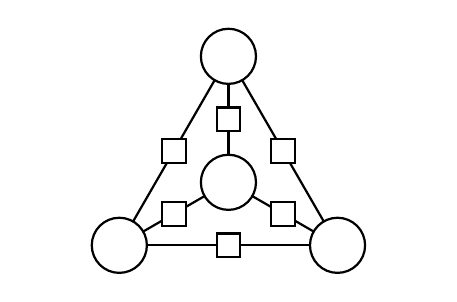
\begin{tikzpicture}
  [normalN/.style={circle,draw,minimum size=0.7cm,fill=white},
   edgeN/.style={draw,minimum size=0.3cm,fill=white},
   thick]

  \coordinate (c) at (0:0);
  \coordinate (t) at (90:1.6);
  \coordinate (l) at (210:1.6);
  \coordinate (r) at (-30:1.6);
  
  \coordinate (cor_tr) at (30:0.8);
  \coordinate (cor_tl) at (150:0.8);
  \coordinate (cor_lr) at (-90:0.8);
  
  \coordinate (cor_ct) at  (90:0.8);
  \coordinate (cor_cl) at (210:0.8);
  \coordinate (cor_cr) at (-30:0.8);

  \draw [] (c) -- (cor_ct); \draw [] (t) -- (cor_ct);
  \draw [] (c) -- (cor_cl); \draw [] (l) -- (cor_cl);
  \draw [] (c) -- (cor_cr); \draw [] (r) -- (cor_cr);
  
  \draw [] (l) -- (cor_lr); \draw [] (r) -- (cor_lr);
  \draw [] (t) -- (cor_tl); \draw [] (l) -- (cor_tl);
  \draw [] (t) -- (cor_tr); \draw [] (r) -- (cor_tr);
  
  \path (210:1.6)+(120:1.6) node[normalN,draw=black!0] (ll) {};
  \path (-30:1.6)+ (60:1.6) node[normalN,draw=black!0] (rr) {};

  \node[normalN]  at   (0:0)   {};
  \node[normalN]  at  (90:1.6) {};
  \node[normalN]  at (210:1.6) {};
  \node[normalN]  at (-30:1.6) {};
  
  \node[edgeN] (etr) at  (cor_tr) {};
  \node[edgeN] (etl) at (150:0.8) {};
  \node[edgeN] (elr) at (-90:0.8) {};

  \node[edgeN] (ect) at  (90:0.8) {};
  \node[edgeN] (ecl) at (210:0.8) {};
  \node[edgeN] (ecr) at (-30:0.8) {};

  %\path (210:1.6)+(120:0.8) node[edgeN] (ell) {};
  %\path (-30:1.6)+ (60:0.8) node[edgeN] (err) {};

  
  %\draw [] (l) -- (ell); \draw [] (ll) -- (ell);
  %\draw [] (r) -- (err); \draw [] (rr) -- (err);
\end{tikzpicture}}
\hspace*{\fill} 
\subfloat[Graph $G_2$]{\begin{tikzpicture}
  [normalN/.style={circle,draw,minimum size=0.7cm,fill=white},
   edgeN/.style={draw,minimum size=0.3cm,fill=white},
   thick]

  \coordinate (c) at (0:0);
  \coordinate (t) at (90:1.6);
  \coordinate (l) at (210:1.6);
  \coordinate (r) at (-30:1.6);
  
  \coordinate (cor_tr) at (30:0.8);
  \coordinate (cor_tl) at (150:0.8);
  \coordinate (cor_lr) at (-90:0.8);
  
  \coordinate (cor_ct) at  (90:0.8);
  \coordinate (cor_cl) at (210:0.8);
  \coordinate (cor_cr) at (-30:0.8);

  \coordinate (cor_ll) at ($(210:1.6)+(120:0.8)$);
  \coordinate (cor_rr) at ($(-30:1.6)+ (60:0.8)$);

  \path (210:1.6)+(120:1.6) node[normalN] (ll) {};
  \path (-30:1.6)+ (60:1.6) node[normalN] (rr) {};
  
  \draw [] (c) -- (cor_ct); \draw [] (t) -- (cor_ct);
  
  \draw [] (l) -- (cor_lr); \draw [] (r) -- (cor_lr);
  \draw [] (t) -- (cor_tl); \draw [] (l) -- (cor_tl);
  \draw [] (t) -- (cor_tr); \draw [] (r) -- (cor_tr);
  
  \draw [] (l) -- (cor_ll); \draw [] (ll) -- (cor_ll);
  \draw [] (r) -- (cor_rr); \draw [] (rr) -- (cor_rr);

  \node[normalN]  at   (0:0)   {};
  \node[normalN]  at  (90:1.6) {};
  \node[normalN]  at (210:1.6) {};
  \node[normalN]  at (-30:1.6) {};
  
  \node[edgeN] (etr) at  (30:0.8) {};
  \node[edgeN] (etl) at (150:0.8) {};
  \node[edgeN] (elr) at (-90:0.8) {};

  \node[edgeN] (ect) at  (90:0.8) {};
  %\node[edgeN] (ecl) at (210:0.8) {};
  %\node[edgeN] (ecr) at (-30:0.8) {};

  \path (210:1.6)+(120:0.8) node[edgeN] (ell) {};
  \path (-30:1.6)+ (60:0.8) node[edgeN] (err) {};

\end{tikzpicture}
}
\hspace*{\fill} \\ \hspace*{\fill} 
\subfloat[MCS von $G_1$ und $G_2$]{\begin{tikzpicture}
  [normalN/.style={circle,draw,minimum size=0.7cm,fill=white},
   edgeN/.style={draw,minimum size=0.3cm,fill=white},
   thick]

  \coordinate (c) at (0:0);
  \coordinate (t) at (90:1.6);
  \coordinate (l) at (210:1.6);
  \coordinate (r) at (-30:1.6);
  
  \coordinate (cor_tr) at (30:0.8);
  \coordinate (cor_tl) at (150:0.8);
  \coordinate (cor_lr) at (-90:0.8);
  
  \coordinate (cor_ct) at  (90:0.8);
  \coordinate (cor_cl) at (210:0.8);
  \coordinate (cor_cr) at (-30:0.8);

  %\path (210:1.6)+(120:1.6) node[normalN] (ll) {};
  %\path (-30:1.6)+ (60:1.6) node[normalN] (rr) {};

  \draw [] (t) -- (cor_ct);
  \draw [] (l) -- (cor_cl);
  \draw [] (r) -- (cor_cr);
  
  \draw [] (l) -- (cor_lr); \draw [] (r) -- (cor_lr);
  \draw [] (t) -- (cor_tl); \draw [] (l) -- (cor_tl);
  \draw [] (t) -- (cor_tr); \draw [] (r) -- (cor_tr);
  
  %\node[normalN] (c) at   (0:0)   {};
  \node[normalN]  at  (90:1.6) {};
  \node[normalN]  at (210:1.6) {};
  \node[normalN]  at (-30:1.6) {};
  
  \node[edgeN] (etr) at  (30:0.8) {};
  \node[edgeN] (etl) at (150:0.8) {};
  \node[edgeN] (elr) at (-90:0.8) {};

  \node[edgeN,draw=darkgreen] (ect) at  (90:0.8) {};
  \node[edgeN,draw=darkgreen] (ecl) at (210:0.8) {};
  \node[edgeN,draw=darkgreen] (ecr) at (-30:0.8) {};

  %\path (210:1.6)+(120:0.8) node[edgeN] (ell) {};
  %\path (-30:1.6)+ (60:0.8) node[edgeN] (err) {};

  
  %\draw [] (l) -- (ell); \draw [] (ll) -- (ell);
  %\draw [] (r) -- (err); \draw [] (rr) -- (err);
\end{tikzpicture}} \hspace*{\fill} 
\caption{Das Phänomen der freien Kanten}
\label{pic:bspFreieKanten}
\end{figure}

\subsubsection{Größe des Kantengraphen}
Ein weiterer Nachteil ist, dass die Knotenzahl deutlich steigt. Da sowohl 
das Ermitteln des MCS als auch des Graphabstands NP-vollständig ist, 
gibt es vermutlich keinen Algorithmus in polynomieller Laufzeit sondern 
nur mit exponentieller. Ein Anstieg der Knoten und Kanten kann sich 
somit deutlich auf die Laufzeit auswirken.

%\section{Cliquen und unabhängige Mengen}
%Cliquen und unabhängige Mengen (engl.: independent set) sind besondere
%Mengen in Graphen. Eine Clique ist ein Graph, dessen Knoten alle miteinander
%verbunden sind. Im Gegensatz dazu ist ein independent set eine Menge von
%Knoten, zwischen denen keine Kante existiert.
%
%\begin{mydef}[Clique]
%Es seien $G=(V,E)$ ein ungerichteter Graph und $C=(V_c,E_c)$ 
%ein Teilgraph von $G$. $C$ ist eine Clique in $G$ genau dann, wenn 
%für alle $u$ und $v$ ($,v \in V_c$; $u\neq v$) gilt: $(u,v) \in E_c$.
%\end{mydef}
%
%\begin{mydef}[independent set]
%Sei $G=(V,E)$ ein ungerichteter Graph. $V_i \subseteq V$ ist
%ein independent set in $G \Leftrightarrow \forall e \in V_i \times 
%V_i: e \notin E$.
%\end{mydef}
%
%\begin{mydef}[Komplementärgraph]
%Sei $G=(V,E)$ ein Graph. $\overline{G}=(V,(V \times V) \backslash E)$ wird 
%als Komplementärgraph von $G$ bezeichnet.
%%ToDo: (u,u) nicht erlauben
%\end{mydef}
%
%Das Finden einer maximalen Clique oder eines maximalen independent sets
%(MIS) sind äquivalente Probleme. Dies liegt daran, dass eine Clique in $G$
%auch automatisch ein independent set im Komplementärgraphen $\overline{G}$
%darstellt. Aus der NP-Vollständigkeit des Findens der maximalen Clique
%\cite{Karp72} folgt somit, dass auch die Ermittlung des maximalen
%independent sets NP-vollständig ist.

\section{MCS und Assoziationsgraphen}\label{sec:MIS_MCS}
Das Finden eines MCS zweier Graphen lässt sich auf die Suche nach 
einer unabhängigen Menge (engl.: independent set) reduzieren \cite{MaxCSwitMaxIS}. 
Dazu erstellt man aus den gegebenen Graphen einen 
Assoziationsgraphen (AG). In diesem sucht man dann nach einem maximalen 
independent set.

\subsection{Unabhängige Menge}
Eine Unabhängige Menge in einem Graphen ist eine Teilmenge der Knoten des 
Graphen, wobei zwischen den Knoten keine Kante vorhanden ist.

\begin{mydef}[independent set]
Sei $G=(V,E)$ ein ungerichteter Graph. $V_i \subseteq V$ ist 
ein independent set in $G$ genau dann, wenn für alle $e \in V_i \times 
V_i$ gilt: $e \notin E$.
\end{mydef}

Das Ermitteln des maximum independent set (MIS) ist NP-vollständig \cite{Garey:1990}.

\subsection{Assoziationsgraph}
Ein gemeinsamer induzierter Teilgraph ist eine Abbildung der Knoten 
von einem Graphen $G_1$ auf die Knoten eines Graphen $G_2$ (siehe Definition \ref{def:gTG}). 
Die Idee des AGs ist es, jede mögliche Zuordnung, die zu einer 
solchen Abbildung gehören kann, in einem Graphen darzustellen.

%\begin{figure}[htb]
%\centering
%\includegraphics[width=0.4\linewidth,keepaspectratio]{bilder/bsg_ag_graphs.png}
%\caption{Die Graphen $G_1$ (oben) und $G_2$ (unten)}
%\label{pic:bsg_ag_graphs}
%\end{figure}

\begin{figure}[htb]
\centering
\vspace{0.5cm}
\begin{tikzpicture}
  [normalN/.style={circle,draw,minimum size=0.8cm,thick},
   node distance=0.8cm]

  \path (0,0)     node[normalN] (a) {a}
       +(0.8,-1.6) node[normalN] (1) {1};
       
  \node[normalN] (b) [right=of a] {b};
  \node[normalN] (c) [right=of b] {c};
  \node[normalN] (2) [right=of 1] {2};
    
  \draw [thick] (a) -- (b);
  \draw [thick] (b) -- (c);
  \draw [thick] (1) -- (2);
    
\end{tikzpicture}
\caption{Die Graphen $G_1$ (oben) und $G_2$ (unten)}
\label{pic:bsg_ag_graphs}
\end{figure}

Die Knoten des AGs stellen die möglichen Zuordnungen von einem Knoten auf 
einen anderen dar. Jeder Knoten ist somit ein Paar aus einem Knoten aus $G_1$ 
und einem Knoten aus $G_2$. Abbildung \ref{pic:bsg_ag_nodes} stellt die Kantenmenge des AGs 
dar, der sich aus den Graphen in Abbildung \ref{pic:bsg_ag_graphs} ergibt.

%\begin{figure}[htb]
%\centering
%\includegraphics[width=0.4\linewidth,keepaspectratio]{bilder/bsg_ag_nodes.png}
%\caption{Die Knoten des Assoziationsgraphen von $G_1$ und $G_2$}
%\label{pic:bsg_ag_nodes}
%\end{figure}

\begin{figure}[htb]
\centering
\vspace{0.5cm}
\begin{tikzpicture}
  [normalN/.style={circle,draw,minimum size=0.8cm,thick},
   node distance=0.8cm]

  \node[normalN] (1a) {1a};
  \node[normalN] (1b) [right=of 1a] {1b}; 
  \node[normalN] (1c) [right=of 1b] {1b};
  \node[normalN] (2a) [below=of 1a] {2a};
  \node[normalN] (2b) [below=of 1b] {2b};
  \node[normalN] (2c) [below=of 1c] {2c};
\end{tikzpicture}
\caption{Die Knoten des Assoziationsgraphen von $G_1$ und $G_2$}
\label{pic:bsg_ag_nodes}
\end{figure}

Die Kanten des AGs (dargestellt in Abbildung \ref{pic:bsg_ag_edges}) geben an, 
ob Knotenpaare (also die Zuordnung eines Knotens zu einem anderen) einander 
ausschließen. Es gibt zwei Fälle, in denen das der Fall ist: 
\begin{itemize}
  \item Ein Knoten $u$ aus $G_1$ kann nur höchstens einmal auf einen anderen 
	      Knoten in $G_2$ abgebildet werden. Alle anderen Knotenpaare, die den 
        Knoten $u$ beinhalten, sind somit nicht mehr möglich. Analog verhalten 
        sich die Knoten aus $G_2$. Sie können nur einmal Ziel einer Zuordnung 
        sein.
        
        Die so erzeugten Kanten sind in Abbildung \ref{pic:bsg_ag_edges} 
        \emph{schwarz} dargestellt.
        
  \item Hat man ein Knotenpaar, so schließt dies weitere Paare 
        aus. Diese Paare ergeben sich durch die Betrachtung der Kanten der beiden 
        ursprünglichen Graphen. Ein Paar $(u_1, u_2)$ schließt ein Paar 
        $(v_1, v_2)$ aus, wenn es eine Kante (in $G_1$) zwischen $u_1$ 
        und $v_1$ gibt, jedoch keine (in $G_2$) zwischen $u_2$ und $v_2$. 
        Dies ist nötig, da ein induzierter Teilgraph dargestellt werden soll.
        
        Die so erzeugten Kanten sind in Abbildung \ref{pic:bsg_ag_edges} 
        \emph{rot} dargestellt.

\end{itemize}

%\begin{figure}[htb]
%\centering
%\includegraphics[width=0.4\linewidth,keepaspectratio]{bilder/bsg_ag_edges.png}
%\caption{Der vollständige Assoziationsgraphen von $G_1$ und $G_2$}
%\label{pic:bsg_ag_edges}
%\end{figure}

\begin{figure}[htb]
\centering
\begin{tikzpicture}
  [normalN/.style={circle,draw,minimum size=0.8cm,thick},
   node distance=0.8cm]

  \node[normalN] (1a) {1a};
    
  \node[normalN] (1b) [right=of 1a] {1b}
     edge [thick] (1a); 
    
  \node[normalN] (1c) [right=of 1b] {1c}
     edge [thick] (1b);
    
  \node[normalN] (2a) [below=of 1a] {2a}
     edge [thick] (1a);
    
  \node[normalN] (2b) [below=of 1b] {2b}
     edge [thick] (1b)
     edge [thick] (2a);
    
  \node[normalN] (2c) [below=of 1c] {2c}
     edge [thick] (1c)
     edge [thick] (2b);
  
  \draw [thick,red] (1a) to (2c);
  \draw [thick,red] (2a) to (1c);
  
  \draw [thick] (1c) .. controls +(135:1.3cm) and +(45:1.3cm) .. (1a);
  \draw [thick] (2c) .. controls +(-135:1.3cm) and +(-45:1.3cm) .. (2a);
\end{tikzpicture}
\caption{Der vollständige Assoziationsgraph von $G_1$ und $G_2$}
\label{pic:bsg_ag_edges}
\end{figure}

Für einen AG ergibt sich somit die folgende (auf der Beschreibung in 
\cite{MaxCSwitMaxIS} basierende) Definition:

\begin{mydef}[Assoziationsgraph]\label{def:Assoziationsgraph}
Gegeben seinen zwei Graphen $G_1=(V_1,E_1)$ und $G_2=(V_2,E_2)$. Ein 
Assoziationsgraph $G_A(G_1,G_2)=(V_A,E_A)$ sei wie folgt definiert:
\begin{itemize}
	\item $V_A= V_1 \times V_2$
	\item $E_A=\{((u_1,u_2),(v_1,v_2))\ |\ u_i=v_i \vee 
	       ((u_1,v_1) \in E_1 \oplus  (u_2,v_2) \in E_2)\}$\footnote{$a \oplus b \equiv
	       (a \wedge \neg b) \vee (\neg a \wedge b)$ -- "`Entweder $a$ oder $b$"'}
\end{itemize}
\end{mydef}

Jedes independent set im AG von $G_1$ und $G_2$ stellt nun einen gemeinsamen 
induzierten Teilgraphen von $G_1$ und $G_2$ dar \cite{MaxCSwitMaxIS}. Somit 
entspricht das MIS des AGs dem MCS von $G_1$ und $G_2$.
